\documentclass[preprint,12pt]{elsarticle}
\usepackage{amsmath}
\usepackage{booktabs}
\usepackage{graphicx}
\usepackage{hyperref}
\usepackage{float}
\usepackage{xcolor}

\journal{Economics Letters}

\begin{document}

\begin{frontmatter}

\title{Mining Deregulation and Homicides: Evidence from Indigenous Territories in Brazil}

\author[u1]{Pedro Hemsley}
\author[u1]{Romero Rocha}
\author[u2]{Victor Libera}
\address[u1]{Universidade Federal do Rio de Janeiro, Brazil}
\address[u2]{Banco Nacional de Desenvolvimento Economico e Social (BNDES), Brazil}

\begin{abstract}
We study whether Brazil's federal enforcement shift against illegal gold mining was associated with higher violence in environmentally sensitive municipalities. We build a municipality-year panel (2010--2022), restrict the sample to municipalities in Amazonia or Cerrado, and combine homicide rates with geospatial indicators for Indigenous-territory overlap and gold-reserve overlap. In a difference-in-differences-in-differences design, municipalities with both characteristics experience a large post-2016 increase in homicide rates. Results are robust to using 2017 as treatment start, to state-by-year fixed effects, to decomposition into simple DDs, to placebo treatment-year tests, and to population-weighted estimation. In dual-break specifications that also include the 2013 deregulation shock emphasized by \citealp{pereira_pucci_2024}, the post-2016 increment remains positive and statistically significant.
\end{abstract}

\begin{keyword}
Illegal mining \sep Indigenous territories \sep Violence \sep Difference-in-differences \sep Brazil
\end{keyword}

\end{frontmatter}

\section{Introduction}
Illegal gold mining in Brazil is concentrated in areas where extraction is legally restricted, especially Indigenous territories. In those areas, high resource rents and contested land rights can intensify violent conflict. We examine whether the federal enforcement shift that begins in the Temer period is associated with higher homicide rates where illegal mining incentives are strongest.

This question connects to the broader literature on commodity incentives, conflict, and local violence (\citealp{dube2013commodity,fetzer2017property,moreno2024technical,falcone2022modernization}).

Our contribution is a compact reduced-form estimate for an \textit{Economics Letters} setting. We focus on municipalities in Amazonia or Cerrado (the biomes most relevant for environmental conflict) and estimate a difference-in-differences-in-differences (DDD) model in annual data from 2010 to 2022. The identifying comparison is between municipalities that simultaneously overlap Indigenous territories and known gold reserves versus municipalities with only one or neither feature.

Our note complements \citealp{pereira_pucci_2024}, who show that the 2013 deregulation of first-buyer liability increased illegal mining and violence in exposed Amazon municipalities. We ask whether a later federal enforcement shift (2016/2017 onward) generated an additional increase in homicides in municipalities where illegal mining incentives are strongest.

The main treatment starts in 2016, when the federal political cycle changes (Temer became interim president on May 12, 2016 and was confirmed on August 31, 2016). We report robustness with treatment starting in 2017.

The timing is also consistent with evidence on weakening environmental enforcement in the Brazilian Amazon after the mid-2010s (\citealp{braganca2022cutting,nunes2024lessons}).

\section{Data and empirical strategy}
\subsection{Data}
We use a municipality-year panel from 2010 to 2022. The outcome is homicide rate per 100,000 inhabitants, constructed from SIM/DATASUS mortality records and official municipal population data.

We combine those data with geospatial indicators:
\begin{itemize}
\item \(TI_i=1\): municipality overlaps at least one official Indigenous territory polygon.
\item \(Gold_i=1\): municipality overlaps known gold-reserve\footnote{\textcolor{red}{In this study, gold-reserve polygons are defined as the spatial intersection of gold provinces and gold districts, whose definitions are presented in \citealp{sgb2022}}} polygons.
\end{itemize}

The sample is restricted to municipalities that overlap Amazonia or Cerrado (any-overlap definition from IBGE municipality-biome correspondence). After missing outcomes and singleton adjustments, the main estimating sample contains 17,524 municipality-year observations.

\subsection{Baseline DDD}
Our baseline specification is
\begin{equation}
y_{it} = \beta_1(Gold_i \times Post_t) + \beta_2(TI_i \times Post_t) + \beta_3(Gold_i \times TI_i \times Post_t) + \mu_i + \lambda_t + \varepsilon_{it},
\end{equation}
where \(y_{it}\) is homicide rate, \(\mu_i\) are municipality fixed effects, and \(\lambda_t\) are year fixed effects. Standard errors are clustered by municipality. The coefficient of interest is \(\beta_3\).

\section{Results}
\subsection{Main estimates}
Table~\ref{tab:main} reports core estimates. In the main model (post-2016), the triple interaction is 8.769 (s.e. 3.419, \(p=0.010\)). With treatment starting in 2017, it is 8.806 (s.e. 3.550, \(p=0.013\)).

Following a concern about flexible differential trends, we estimate non-linear state trends via state-by-year fixed effects. The post-2016 triple interaction remains positive and statistically significant: 9.711 (s.e. 3.470, \(p=0.005\)).

\begin{table}[H]
\caption{Main DDD estimates in Amazonia+Cerrado municipalities (2010--2022)}
\label{tab:main}
\centering
\footnotesize
\setlength{\tabcolsep}{3.5pt}
\renewcommand{\arraystretch}{0.95}
\resizebox{\textwidth}{!}{%\begin{tabular}{lccc}
%\toprule
%& \multicolumn{3}{c}{Dependent variable: Homicide rate per 100,000} \\
%\cmidrule(lr){2-4}
%& Post>=2016 & Post>=2017 & Post>=2016 + state-year FE \\
%& (1) & (2) & (3) \\
%\midrule
%Gold $\times$ Post & 2.529* & 2.886** & 1.750 \\
% & (1.332) & (1.388) & (1.354) \\
%TI $\times$ Post & -0.152 & 0.414 & -2.381* \\
% & (1.133) & (1.118) & (1.394) \\
%Gold $\times$ TI $\times$ Post & 8.769** & 8.806** & 9.711*** \\
% & (3.419) & (3.550) & (3.470) \\
%\midrule
%Municipality FE & Yes & Yes & Yes \\
%Year FE & Yes & Yes & No \\
%State-year FE & No & No & Yes \\
%Observations & 17524 & 17524 & 17511 \\
%Within R\textsuperscript{2} & 0.007 & 0.008 & 0.005 \\
%\midrule
%\multicolumn{4}{l}{\footnotesize Clustered standard errors by municipality in parentheses.} \\
%\multicolumn{4}{l}{\footnotesize *** p<0.01, ** p<0.05, * p<0.1.} \\
%\bottomrule
%\end{tabular}

{\fontsize{7}{8}\selectfont
\begin{tabular}{lccc}
\toprule
& \multicolumn{3}{c}{Dependent Variable: Homicide Rate per 100,000} \\
\cmidrule(lr){2-4}
& Post $\geq$ 2016 & Post $\geq$ 2017 & \makecell{Post $\geq$ 2016 $+$ \\ State-year FE} \\
& (1) & (2) & (3) \\
\midrule
Gold $\times$ Post & 2.662** & 2.761** & 0.884 \\ 
& (1.065) & (1.138) & (1.125) \\
IT $\times$ Post & -0.343 & 0.214 & -2.673** \\
& (1.005) & (0.989) & (1.202) \\
Gold $\times$ IT $\times$ Post & 7.211*** & 7.767*** & 8.691*** \\
 & (2.757) & (2.947) & (2.727) \\
\midrule
Municipality FE & Yes & Yes & Yes \\
Year FE & Yes & Yes & No \\
State-year FE & No & No & Yes \\
Observations & 24,358 & 24,358 & 24,358 \\
\midrule
\multicolumn{4}{l}{ Standard errors in parentheses.} \\
\multicolumn{4}{l}{ *** p $<$ 0.01, ** p $<$ 0.05, * p $<$ 0.1.} \\
\bottomrule
\end{tabular}
}}
\end{table}

To improve interpretation, we decompose the DDD into simple DDs. Within \(TI=1\) municipalities, the DD effect of \(Gold\times Post2016\) is 11.322 (\(p<0.001\)), while within \(TI=0\) it is 2.521 (\(p=0.059\)). Symmetrically, within \(Gold=1\), the DD effect of \(TI\times Post2016\) is 8.561 (\(p=0.008\)), versus -0.138 (\(p=0.903\)) within \(Gold=0\). This pattern is consistent with the DDD estimate.

Additional robustness checks are also supportive. Population-weighted DDD estimates are 9.652 (\(p=0.015\)) with municipality and year FE, and 7.436 (\(p=0.043\)) with municipality and state-by-year FE. Placebo treatment-year tests on pre-period data only (fake starts in 2013 and 2014) are statistically null (\(p=0.449\) and \(p=0.959\)).

To separate our estimates from the 2013 deregulation channel, we estimate dual-break specifications including both post-2013 and post-2016 (or post-2017) interactions. In the 2013+2016 model, the 2013--2015 effect is small and imprecise (2.398, \(p=0.345\)), while the incremental post-2016 effect is 7.600 (\(p=0.025\)); the total post-2016 effect is 9.998 (\(p=0.011\)). With municipality and state-by-year FE, the incremental post-2016 effect is 8.892 (\(p=0.012\)) and the total post-2016 effect is 10.583 (\(p=0.006\)). Using 2017 as the second break yields similar incremental effects (7.464, \(p=0.030\), baseline FE; 8.683, \(p=0.017\), state-by-year FE).

\subsection{Dynamic evidence and pre-trends}
Figure~\ref{fig:event} shows dynamic DDD coefficients for the triple interaction, with 2015 as reference year. Coefficients for 2010--2014 are jointly insignificant in both baseline and state-year FE specifications (\(p=0.892\) and \(p=0.952\)). Post-treatment effects are strongest in 2018 (13.481, \(p=0.003\)) and remain positive in subsequent years, though less precisely estimated.

\begin{figure}[H]
\centering
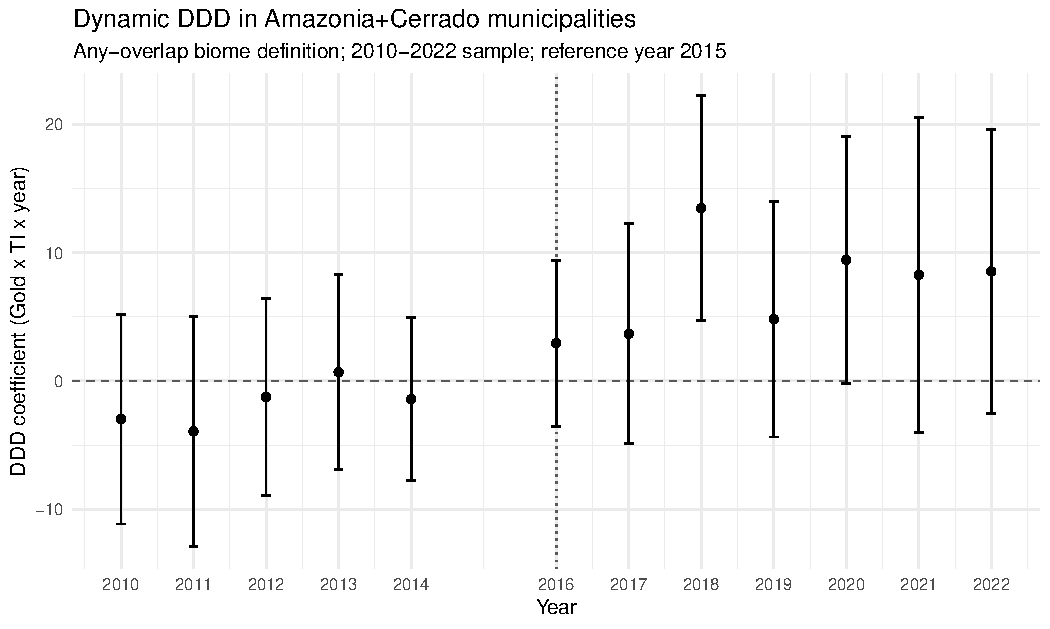
\includegraphics[width=0.88\textwidth]{figures/fig_event_study_ddd.pdf}
\caption{Dynamic DDD event-study (reference year: 2015)}
\label{fig:event}
\end{figure}

\section{Conclusion}
In municipalities located in Amazonia or Cerrado, homicide rates rose after the 2016 federal enforcement shift specifically where Indigenous-territory overlap and gold-reserve overlap coexist. The result is robust to treatment-year coding (2016 vs. 2017), to non-linear state trends, to decomposition into simple DDs, to placebo treatment timing, and to population-weighted estimation.

Dual-break results indicate that this pattern is not mechanically capturing the 2013 deregulation effect documented by \citealp{pereira_pucci_2024}: once both breaks are included, the incremental post-2016/post-2017 effect remains large and significant.

This evidence is consistent with the view that weaker effective enforcement in environmentally sensitive and resource-rich territories can generate substantial local violence costs.

\section*{Data availability}
Data and replication files are available from the authors upon request.

\bibliographystyle{elsarticle-harv}
\bibliography{references}

\end{document}
